\documentclass[xcolor=x11names,compress]{beamer}

%% General document %%%%%%%%%%%%%%%%%%%%%%%%%%%%%%%%%%
\usepackage{graphicx}
\usepackage{tikz}
\usetikzlibrary{decorations.fractals}
\usepackage{mathpazo}
\usepackage[english]{babel}
\usepackage[T1]{fontenc}
\usepackage[utf8]{inputenc}
\usepackage{siunitx}
\usepackage{graphicx}
\usepackage{physics}
\usepackage{multimedia}
\usepackage{subfigure}
\usepackage{xcolor}
\usepackage[absolute,overlay]{textpos}
\usepackage{ragged2e}
\usepackage{amssymb}
\usepackage[version=4]{mhchem}


\renewcommand{\thefootnote}{\alph{footnote}}
%%%%%%%%%%%%%%%%%%%%%%%%%%%%%%%%%%%%%%%%%%%%%%%%%%%%%%


%% Beamer Layout %%%%%%%%%%%%%%%%%%%%%%%%%%%%%%%%%%
\useoutertheme[subsection=false,shadow]{miniframes}
\useinnertheme{default}


\setbeamerfont{title like}{shape=\scshape}
\setbeamerfont{frametitle}{shape=\scshape}
\setbeamerfont{framesubtitle}{size=\normalsize}
\setbeamerfont{caption}{size=\scriptsize}
\setbeamercolor*{lower separation line head}{bg=DeepSkyBlue4} 
\setbeamercolor*{normal text}{fg=black,bg=white} 
\setbeamercolor*{alerted text}{fg=red} 
\setbeamercolor*{example text}{fg=black} 
\setbeamercolor*{structure}{fg=black} 

 
\setbeamercolor*{palette tertiary}{fg=black,bg=black!10} 
\setbeamercolor*{palette quaternary}{fg=black,bg=black!10} 
\setbeamercolor{caption name}{fg=DeepSkyBlue4}
\setbeamercolor{title}{fg=DeepSkyBlue4}
\setbeamercolor{itemize item}{fg=DeepSkyBlue4}
\setbeamercolor{frametitle}{fg=DeepSkyBlue4}
\renewcommand{\(}{\begin{columns}}
\renewcommand{\)}{\end{columns}}
\newcommand{\<}[1]{\begin{column}{#1}}
\renewcommand{\>}{\end{column}}
%%%%%%%%%%%%%%%%%%%%%%%%%%%%%%%%%%%%%%%%%%%%%%%%%%


\setbeamertemplate{navigation symbols}{} 
\setbeamertemplate{footline}[frame number]
\setbeamertemplate{caption}[numbered]
\setbeamertemplate{section in toc}[ball]
\setbeamertemplate{itemize items}[circle]
\beamerboxesdeclarecolorscheme{clair}{Coral4}{Ivory2}
\beamerboxesdeclarecolorscheme{foncé}{DarkSeaGreen4}{Ivory2}

\title[Title]{Perturbative theories in the complex plane}
\author[]{Antoine \textsc{Marie}}
\date{30 Juin 2020}
  \setbeamersize{text margin left=5mm}
  \setbeamersize{text margin right=5mm}
\institute{Supervised by Pierre-François \textsc{LOOS}} 

\begin{document}


%%%%%%%%%%%%%%%%%%%%%%%%%%%%%%%%%%%%%%%%%%%%%%%%%%%%%%
%%%%%%%%%%%%%%%%%%%%%%%%%%%%%%%%%%%%%%%%%%%%%%%%%%%%%%

\begin{frame}[plain]

\date{24 Avril 2020}
\titlepage
\end{frame}

%%%%%%%%%%%%%%%%%%%%%%%%%%%%%%%%%%%%%%%%%%%%%%%%%%%%%%
%%%%%%%%%%%%%%%%%%%%%%%%%%%%%%%%%%%%%%%%%%%%%%%%%%%%%%

\section{\textsc{Strange behaviors of the MP series}}

\begin{frame}{The Möller-Plesset theory}

\begin{beamerboxesrounded}[scheme=foncé]{\centering Partitioning of the Hamiltonian}

\begin{equation}
   H = H_0 + \lambda V
\end{equation}

\end{beamerboxesrounded}

\begin{itemize}
\centering
    \item $H_0$ : Unperturbed Hamiltonian
    \item $V$ : Perturbation operator
\end{itemize}

\begin{beamerboxesrounded}[scheme=foncé]{\centering The Fock operator}

\begin{equation}
   F = T + J + K
\end{equation}
\end{beamerboxesrounded}

\begin{itemize}
\centering
    \item $T$ : Kinetic energy operator
    \item $J$ : Coulomb operator
    \item $K$ : Exchange operator
\end{itemize}
    
\end{frame}

\begin{frame}{Deceptive or slow convergences}

\begin{figure}
    \centering
    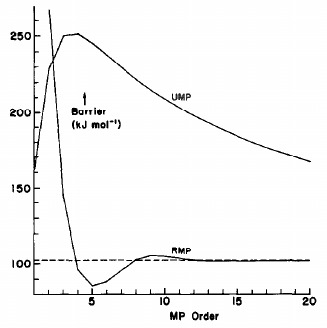
\includegraphics[width=0.5\textwidth]{gill1986.png}
    \caption{\centering Barriers to homolytic fission of \ce{He2^2+} using minimal basis set MPn theory (n~=~1-20).}
    \label{fig:my_label}
\end{figure}

\footnotetext{\tiny{Gill et al.~Deceptive convergence in Møller-Plesset perturbation  energies, \textit{Chemical Physics Letter}, 1986}}
    
\end{frame}

\begin{frame}{Multi-reference and spin contamination}
\begin{table}
    \centering
    \begin{tabular}{c c c c c c c}
\hline
 $r$ & UHF & UMP2 & UMP3 & UMP4 & $<S^2>$ \\
\hline
0.75 & 0.0\% & 63.8\% & 87.4\% & 95.9\% & 0.00\\
1.35 & 0.0\% & 15.2\% & 26.1\% & 34.9\% & 0.49\\
2.00 & 0.0\% & 01.0\% & 01.8\% & 02.6\% & 0.95\\
2.50 & 0.0\% & 00.1\% & 00.3\% & 00.4\% & 0.99\\
\hline
\end{tabular}
    \caption{\centering Percentage of electron correlation energy recovered and $<S^2>$ for the \ce{H2} molecule as a function of bond length (r,A) in the minimal basis.}
    \label{tab:my_label}
\end{table}

\footnotetext{\tiny{Gill et al. Why does unrestricted Møller–Plesset perturbation theory converge so slowly for spin-contaminated wave functions, \textit{Journal of chemical physics}, 1988}}
    
\end{frame}

\begin{frame}{Divergent cases}
  
\begin{figure}
    \centering
    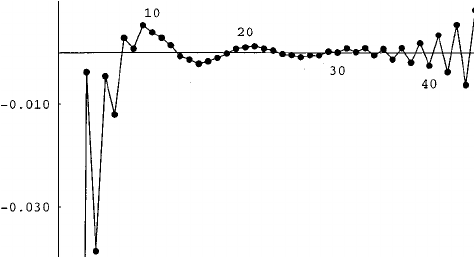
\includegraphics[width=0.6\textwidth]{The-energy-corrections-for-HF-at-stretched-geometry-in-the-cc-pVDZ-basis.png}
    \caption{The energy corrections for HF at stretched geometry in the cc-pVDZ basis.}
    \label{fig:my_label}
\end{figure}
    
\footnotetext{\tiny{Olsen et al. Divergence in Møller–Plesset theory: A simple explanation based on a two-state model, \textit{Journal of chemical physics}, 2000}} 

\end{frame}

\section{The complex plane}

\begin{frame}{A simple example}

\begin{columns}

\column{0.48\textwidth}

\begin{beamerboxesrounded}[scheme=foncé]{An example function}

\begin{equation*}
   \frac{1}{1 + x^4}
\end{equation*}

\end{beamerboxesrounded}

\vspace{1cm}

\begin{itemize}
    \item Smooth for $x \in \mathbb{R}$
    
    \item Infinitely differentiable on $\mathbb{R}$
\end{itemize}

\column{0.48\textwidth}

    \begin{figure}
    \centering
    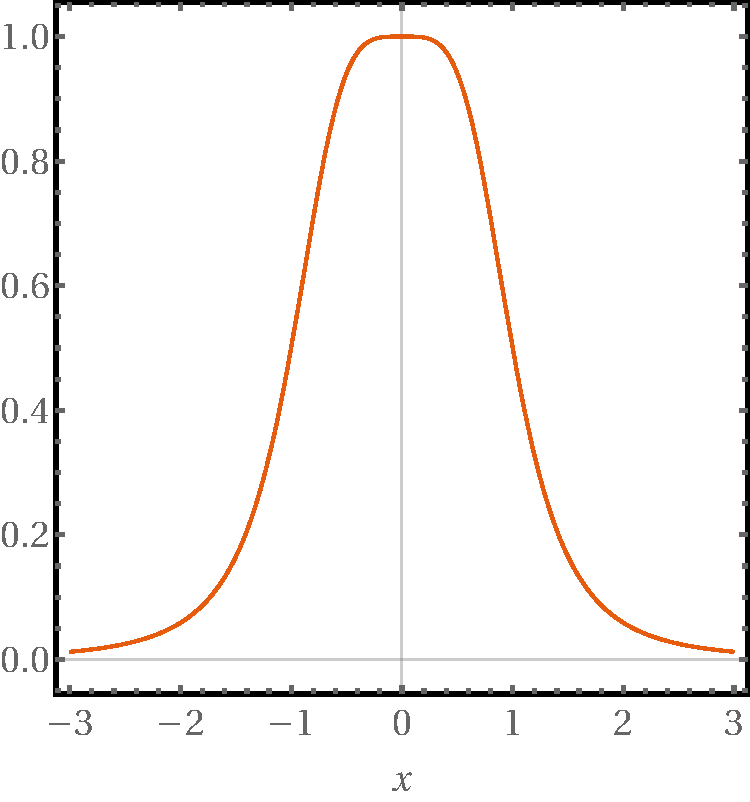
\includegraphics[width=0.6\textwidth]{exemplesingu.pdf}
    \caption{Plot of $1/(1+x^4)$}
    \label{fig:my_label}
\end{figure}

\end{columns}

But the Taylor expansion of this function does not converge for $x\geq1$ ... 
\vspace{0.3cm}
\centering Why ?

\end{frame}

\begin{frame}{And if we look in the complex plane ?}

\begin{columns}

\column{0.48\textwidth}

\centering The function has 4 singularities in the complex plane !

\vspace{1cm}

$x = e^{i\pi/4}, e^{-i\pi/4}, e^{i3\pi/4}, e^{-i3\pi/4}$



\column{0.48\textwidth}

\begin{figure}
    \centering
    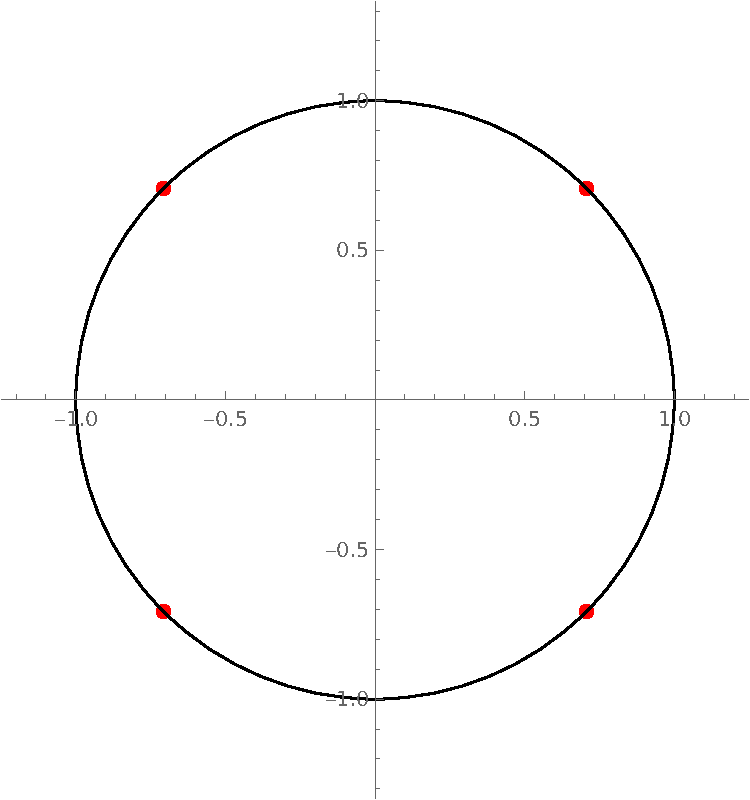
\includegraphics[width=0.6\textwidth]{possingu.pdf}
    \caption{\centering Singularities of the function $1/(1+x^4)$}
    \label{fig:my_label}
\end{figure}

\end{columns}

The \textcolor{red}{radius of convergence} of the Taylor expansion of a function is equal to the distance of the \textcolor{red}{closest singularity} to the origin in the \textcolor{red}{complex plane}.
    
\end{frame}

\begin{frame}{Extending chemistry in the complex plane}

\begin{beamerboxesrounded}[scheme=foncé]{\centering $\lambda$ a complex variable}

\begin{equation*}
   H = H_0 + \lambda V
\end{equation*}

\end{beamerboxesrounded}

\begin{columns}

\column{0.48\textwidth}

\begin{itemize}
    \item $n$ Riemann sheets
    \vspace{0.3cm}
    \item Exceptional points interconnecting the sheets
    \vspace{0.3cm}
    \item No ordering property in the complex plane
\end{itemize}

\column{0.48\textwidth}

\begin{figure}
    \centering
    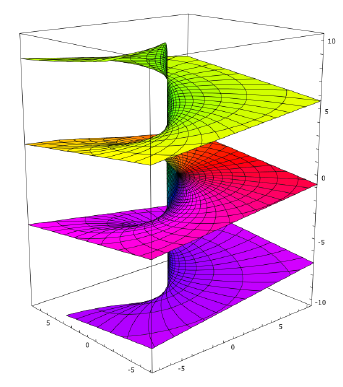
\includegraphics[width=0.7\textwidth]{riemannsheet.png}
    \label{fig:my_label}
\end{figure}

\end{columns}

\end{frame}

\section{Classifying the singularity}

\begin{frame}{Which features of the system localize the singularities ?}

\begin{itemize}
    \item Partitioning of the Hamiltonian: Möller-Plesset, Epstein-Nesbet, ...
    \item Zeroth order reference: weak correlation or strongly correlated electrons.
    \item Finite or complete basis set.
    \item Localized or delocalized basis functions.
\end{itemize}
    
\end{frame}

\begin{frame}{A two-state model}

\begin{columns}

\column{0.48\textwidth}

\begin{figure}
    \centering
    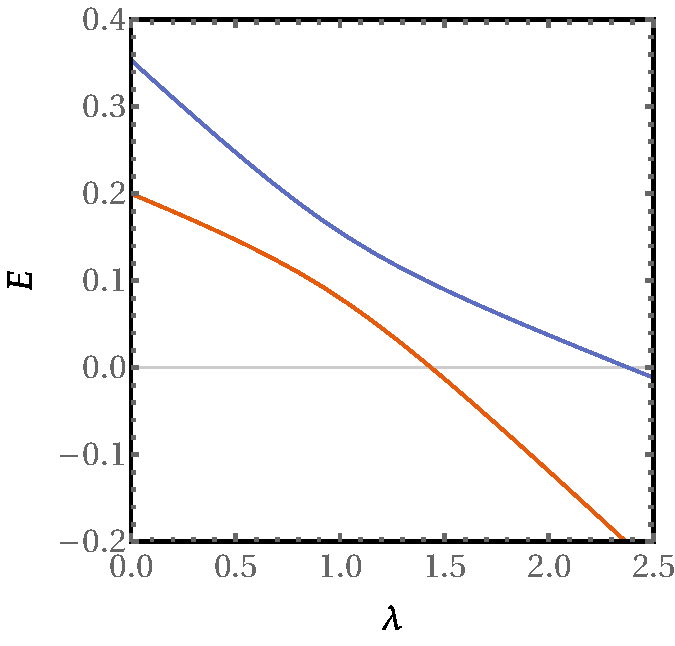
\includegraphics[width=0.8\textwidth]{avoidedcrossing.pdf}
    \caption{Example of an avoided crossing.}
    \label{fig:my_label}
\end{figure}

\column{0.48\textwidth}

\begin{beamerboxesrounded}[scheme=foncé]{A 2x2 matrix\textsuperscript{a}}

$

\small{\centering \begin{pmatrix}
   \alpha & \delta \\
   \delta & \beta 
\end{pmatrix} = 

\vspace{0.3cm}

\begin{pmatrix}

   \alpha + \alpha_s & 0 \\
   0 & \beta + \beta_s
\end{pmatrix} +
\begin{pmatrix}
   - \alpha_s & \delta \\
   \delta & - \beta_s
\end{pmatrix}}
$

\end{beamerboxesrounded}
\vspace{1cm}
\end{columns}

\footnotetext{\tiny{Olsen et al. Divergence in Møller–Plesset theory: A simple explanation based on a two-state model, \textit{Journal of chemical physics}, 2000}} 
    
\end{frame}

\begin{frame}{Two state model}
  
\begin{figure}
    \centering
    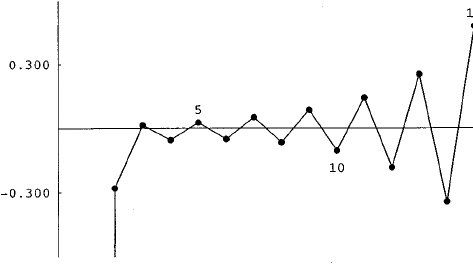
\includegraphics[width=0.6\textwidth]{figure-fig14.png}
    \caption{\centering The energy corrections for HF at stretched geometry in the aug'-cc-pVDZ basis with the two-state model.\textsuperscript{a}}
    \label{fig:my_label}
\end{figure}
    
\footnotetext{\tiny{Olsen et al. Divergence in Møller–Plesset theory: A simple explanation based on a two-state model, \textit{Journal of chemical physics}, 2000}} 

\end{frame}

\begin{frame}{Existence of a critical point}

For $\lambda<0$ :

\begin{equation*}
    H(\lambda)=\sum\limits_{j=1}^{2n}\left[ \underbrace{-\frac{1}{2}\nabla_j^2 - \sum\limits_{k=1}^{N} \frac{Z_k}{|\vb{r}_j-\vb{R}_k|}}_{\text{Independant of }\lambda} + \overbrace{(1-\lambda)V_j^{(scf)}}^{\textcolor{red}{Repulsive}}+\underbrace{\lambda\sum\limits_{j<l}^{2n}\frac{1}{|\vb{r}_j-\vb{r}_l|}}_{\textcolor{blue}{Attractive}}  \right]
\end{equation*}

\end{frame}

\begin{frame}{Critical point in a finite basis set}
    
\begin{beamerboxesrounded}[scheme=foncé]{\centering Exact energy $E(z)$}
$E(z)$ has a critical point on the negative real axis and $E(z)$ is continue for real value below $z_{crit}$.
\end{beamerboxesrounded}

\vspace{0.5cm}

\begin{beamerboxesrounded}[scheme=foncé]{\centering In a finite basis set}
The singularities occur in complex conjugate pairs with non-zero imaginary parts and the energies are discrete. 
\end{beamerboxesrounded}

\vspace{0.5cm}

\centering \Large{How is this connected ???}
    
\end{frame}

\begin{frame}{Singularities $\alpha$ and $\beta$}

\begin{beamerboxesrounded}[scheme=foncé]{\centering Observation}
We can separate singularities in two parts. 
\end{beamerboxesrounded}    

\begin{beamerboxesrounded}[scheme=foncé]{\centering Singularity $\alpha$}
\begin{itemize}
    \item Large avoided crossing
    \item Interaction with a low lying doubly excited states
    \item Non-zero imaginary part
\end{itemize} 
\end{beamerboxesrounded}  

\begin{beamerboxesrounded}[scheme=foncé]{\centering Singularity $\alpha$}
\begin{itemize}
    \item Sharp avoided crossing
    \item Interaction with a diffuse function 
    \item Very small imaginary part
\end{itemize} 
\end{beamerboxesrounded} 

\end{frame}

\begin{frame}{Modeling the critical point}
    
\end{frame}

\section{The spherium model}

\begin{frame}{Spherium: a theoretical playground}

\begin{beamerboxesrounded}[scheme=foncé]{\centering Two electrons on a sphere Hamiltonian}
\begin{equation*}
    H=-\frac{1}{2}(\nabla_1^2 + \nabla_2^2) + \frac{1}{r_{12}}
\end{equation*} 
\end{beamerboxesrounded}
\vspace{0.5cm}

\begin{columns}

\column{0.48\textwidth}

\centering{Small $R$}
\vspace{0.5cm}

\begin{itemize}
    \item $E_{kin} >> E_p$
    \item Uniform density of electrons
    \item \textcolor{red}{Weak correlation}
\end{itemize}

\vspace{0.5cm}

\column{0.48\textwidth}

\centering{Large $R$}
\vspace{0.5cm}

\begin{itemize}
    \item $E_{kin} << E_p$
    \item Electrons on the opposite sides of the sphere
    \item \textcolor{red}{Strong correlation}
    \end{itemize}

\end{columns}

\end{frame}

\begin{frame}{Why is there a class $\beta$ singularity ?}
    
\end{frame}

\begin{frame}{Conclusion}
    
\end{frame}

\end{document}